\chapter{Les multiplets de \texorpdfstring{\(SU(5)\)}{SU(5)}, les bosons de jauge leptoquarks et la désintégration du proton}

\lectureoverview{La grande unification devient concrète lorsque le groupe du Modèle standard est inclus dans \(SU(5)\). Pour comprendre ce que cela signifie, nous commençons par établir les éléments nécessaires de la théorie des représentations : la représentation définissante \(N\), sa conjuguée \(\overline N\), les produits tensoriels, les tenseurs symétriques et antisymétriques, ainsi que la représentation adjointe. Une famille du Modèle standard se regroupe alors dans la combinaison étonnamment économique \(\overline{\mathbf 5}\oplus\mathbf{10}\). La même symétrie qui rend cette organisation élégante impose aussi l’existence de bosons de jauge colorés qui transforment les quarks en leptons. Leur échange permet la désintégration du proton, ce qui contraint l’échelle d’unification à se situer vers \(10^{15}\)--\(10^{16}\,\mathrm{GeV}\). L’évolution des couplages de jauge suggère une échelle comparable, et la supersymétrie revient à la fin, car elle rend leur convergence numérique nettement plus précise.}

\section{Pourquoi commencer par les représentations de groupe ?}

Il existe de nombreuses théories de grande unification proposées. Plutôt que de les passer en revue, nous allons examiner un exemple et poser trois questions : qu’est-ce qui le fait fonctionner, quelles nouvelles particules exige-t-il, et comment les expériences le mettent-elles en difficulté ? Le groupe est \(SU(5)\), et sa caractéristique structurelle essentielle est l’inclusion
\begin{equation}
SU(3)_c\times SU(2)_L\times U(1)_Y
\subset SU(5).
\label{eq:l10-sm-embedding}
\end{equation}
Ici, \(SU(3)_c\) agit sur la couleur, \(SU(2)_L\) sur l’isospin faible et \(U(1)_Y\) sur l’hypercharge.

La supersymétrie n’est pas une prémisse de cette construction. Ni la supersymétrie ni la grande unification n’impliquent logiquement l’autre. Leur lien dans ce cours est numérique : lorsqu’on inclut le spectre des superpartenaires dans le calcul du groupe de renormalisation, les trois couplages de jauge se rapprochent davantage d’une valeur commune.

Les particules qu’une symétrie mélange entre elles forment une représentation du groupe de symétrie. Il faut donc d’abord quelques notions de théorie des représentations pour classer les multiplets de particules unifiées.

\subsection{L’exemple familier de \texorpdfstring{\(SU(2)\)}{SU(2)}}

Le groupe \(SU(2)\) associé au moment cinétique ordinaire est étroitement lié aux rotations de l’espace tridimensionnel. Plus précisément, \(SU(2)\) est le revêtement double de \(SO(3)\). Ses représentations irréductibles sont indexées par
\begin{equation}
j=0,\frac12,1,\frac32,\ldots,
\qquad
\dim(j)=2j+1.
\label{eq:l10-su2-spins}
\end{equation}
Ainsi, un scalaire est un singulet, une particule de spin \(\tfrac12\) est un doublet et une particule de spin un est un triplet. Le groupe faible \(SU(2)_L\) est une symétrie physique différente, bien que sa théorie des groupes abstraite soit la même.

\section{La représentation définissante et sa conjuguée}

Pour \(SU(N)\), la représentation définissante est l’espace des colonnes complexes à \(N\) composantes,
\begin{equation}
\psi=
\begin{pmatrix}
\psi_1\\
\psi_2\\
\vdots\\
\psi_N
\end{pmatrix},
\qquad
\psi'_i=U_i{}^j\psi_j,
\qquad
U\in SU(N).
\label{eq:l10-defining}
\end{equation}
On l’appelle représentation définissante ou, plus simplement, \(\mathbf N\). Les matrices \(U\) sont de taille \(N\times N\), et l’espace vectoriel sur lequel elles agissent est de dimension \(N\).

La conjugaison complexe fournit une autre représentation de dimension \(N\),
\begin{equation}
\psi_i^*\longmapsto U_i{}^{j*}\psi_j^*,
\label{eq:l10-conjugate}
\end{equation}
notée \(\overline{\mathbf N}\). Pour \(N>2\), les représentations définissante et conjuguée ne sont pas équivalentes. On peut intervertir les appellations de représentation des particules et des antiparticules, mais une fois la convention choisie, il faut la conserver.

\begin{classroomqa}
\audiencequestion{Le \(N\) dans \(SU(N)\) dépend-il du fait que \(N\) soit pair ou impair, et désigne-t-il les matrices ? \lecturetimestamp{00:07:33}}
\lecturerresponse{Il n’y a ici aucune restriction de parité --. \(N\) désigne la taille des matrices définissantes et aussi la dimension de leur représentation définissante. \(\mathbf N\) et \(\overline{\mathbf N}\) ont toutes deux cette dimension.}
\end{classroomqa}

L’antiparticule d’une antiparticule est la particule initiale. C’est pourquoi intervertir les appellations \(\mathbf N\) et \(\overline{\mathbf N}\) revient à changer de convention, et non de physique.

\section{Produits tensoriels et irréductibilité}

Supposons qu’un objet puisse occuper \(N\) états internes et qu’un autre puisse indépendamment en occuper autant. Si l’on fait abstraction de la position, de la quantité de mouvement, du spin et de tous les nombres quantiques à l’exception de cet indice \(SU(N)\), la paire possède
\begin{equation}
N\times N=N^2
\label{eq:l10-product-count}
\end{equation}
états. Si le premier objet est dans l’état \(\psi_i\) et le second dans l’état \(\phi_j\), leur produit peut s’écrire
\begin{equation}
\Psi_{ij}=\psi_i\phi_j,
\qquad
\Psi'_{ij}=U_i{}^kU_j{}^\ell\Psi_{k\ell}.
\label{eq:l10-tensor-transform}
\end{equation}
C’est le produit tensoriel \(\mathbf N\otimes\mathbf N\).

\begin{classroomqa}
\audiencequestion{Pourquoi obtient-on \(N^2\) plutôt que \(N^2-1\), et le fait d’autoriser les deux particules à avoir le même indice interne viole-t-il le principe d’exclusion ? \lecturetimestamp{00:10:22}}
\lecturerresponse{Les deux emplacements sont ici distinguables : un objet est fixé à une position et l’autre à une autre. Le principe de Pauli porte sur l’état quantique complet, position comprise. Il n’élimine aucune de ces \(N^2\) combinaisons d’indices internes. Le nombre \(N^2-1\) apparaîtra plus tard, à la suite d’une condition de trace nulle dans un autre produit.}
\end{classroomqa}

La représentation produit de dimension \(N^2\) est en général réductible. Une représentation est réductible lorsqu’elle contient un sous-espace propre que le groupe laisse invariant. On peut isoler ces sous-espaces invariants et les traiter comme des représentations plus petites ; en l’absence d’un tel sous-espace propre, la représentation est irréductible.

\subsection{Tenseurs symétriques et antisymétriques}

Tout tenseur à deux indices se décompose de manière unique en
\begin{align}
\Psi_{ij}
&=\Psi^{(S)}_{ij}+\Psi^{(A)}_{ij},\\
\Psi^{(S)}_{ij}
&=\frac12(\Psi_{ij}+\Psi_{ji}),\\
\Psi^{(A)}_{ij}
&=\frac12(\Psi_{ij}-\Psi_{ji}).
\label{eq:l10-sym-anti}
\end{align}
Les deux termes vérifient
\begin{equation}
\Psi^{(S)}_{ij}=\Psi^{(S)}_{ji},
\qquad
\Psi^{(A)}_{ij}=-\Psi^{(A)}_{ji}.
\end{equation}
L’équation~\eqref{eq:l10-tensor-transform} préserve chacune de ces conditions : les transformations du groupe ne mélangent donc jamais les secteurs symétrique et antisymétrique.

\editorialnote{Le cours laisse le dénombrement général en exercice. Les dimensions des secteurs symétrique et antisymétrique sont respectivement \(N(N+1)/2\) et \(N(N-1)/2\), et leur somme vaut \(N^2\).}

\begin{figure}[htbp]
\centering
\includegraphics[width=0.78\textwidth]{lecture_10_figure_02.png}
\lectureframe{00:17:57.500}
\caption{La décomposition complète au tableau des états de spin \(\tfrac12\) : trois états symétriques et un état antisymétrique.}
\label{fig:l10-spin-decomposition}
\end{figure}

Pour le doublet définissant de \(SU(2)\),
\begin{equation}
\mathbf2\otimes\mathbf2=\mathbf3_S\oplus\mathbf1_A.
\label{eq:l10-two-two}
\end{equation}
En notant les deux états de base \(u\) et \(d\), le triplet symétrique est
\begin{align}
\ket{1,1}&=\ket{uu},\\
\ket{1,0}&=\frac{1}{\sqrt2}\bigl(\ket{ud}+\ket{du}\bigr),\\
\ket{1,-1}&=\ket{dd},
\end{align}
tandis que le singulet antisymétrique est
\begin{equation}
\ket{0,0}
=\frac{1}{\sqrt2}\bigl(\ket{ud}-\ket{du}\bigr).
\end{equation}
C’est l’addition familière de deux moments cinétiques de spin \(\tfrac12\) : les quatre états bruts se réorganisent en un état de spin un et un état de spin zéro.

\section{Une particule et une antiparticule : la représentation adjointe}

Combinons maintenant la représentation définissante avec sa conjuguée. Le produit comporte toujours \(N^2\) composantes, mais se transforme comme une matrice :
\begin{equation}
M_i{}^j\in\mathbf N\otimes\overline{\mathbf N},
\qquad
M\longmapsto U M U^\dagger.
\label{eq:l10-matrix-transform}
\end{equation}
Contrairement à \(\mathbf N\otimes\mathbf N\), il n’y a pas de symétrie d’échange pertinente entre un indice fondamental et un indice antifondamental. La décomposition naturelle est plutôt
\begin{equation}
M
=
\frac{\operatorname{tr}M}{N}\,\mathbf1_N
+
\left(M-\frac{\operatorname{tr}M}{N}\,\mathbf1_N\right).
\label{eq:l10-trace-split}
\end{equation}
Le premier terme est un singulet et la partie sans trace est la représentation adjointe :
\begin{equation}
\mathbf N\otimes\overline{\mathbf N}
=\mathbf1\oplus\mathbf{Adj},
\qquad
\dim\mathbf{Adj}=N^2-1.
\label{eq:l10-adjoint}
\end{equation}

\begin{figure}[htbp]
\centering
\includegraphics[width=0.67\textwidth]{lecture_10_figure_04.png}
\lectureframe{00:23:47.500}
\caption{Conclusion au tableau pour \(\mathbf N\otimes\overline{\mathbf N}\) : ses \(N^2-1\) composantes sans trace forment la représentation adjointe.}
\label{fig:l10-adjoint}
\end{figure}

Pour \(SU(3)\), on obtient l’octet familier,
\begin{equation}
\mathbf3\otimes\overline{\mathbf3}
=\mathbf8\oplus\mathbf1,
\end{equation}
et les huit gluons se transforment selon la représentation adjointe. Pour \(SU(2)\), la représentation adjointe est de dimension trois et se transforme comme un spin un.

\section{Une famille du Modèle standard}

On observe trois générations, mais \(SU(5)\) reproduit la même construction séparément pour chacune. Il n’explique pas pourquoi il y a trois copies. Nous nous concentrons donc sur la première génération.

Tous les champs seront écrits comme des champs de Weyl gauches. Un fermion droit est représenté par son champ conjugué de charge gauche :
\begin{equation}
u^c_L,\qquad d^c_L,\qquad e^c_L.
\label{eq:l10-left-handed-bookkeeping}
\end{equation}
L’exposant \(c\) indique la conjugaison de charge ; par exemple, \(d^c_L\) est un champ anti-down gauche de charge électrique \(+\tfrac13\).

Dans la notation standard de \(SU(5)\), cinq des quinze champs gauches s’insèrent dans
\begin{equation}
\overline{\mathbf5}
=
\begin{pmatrix}
\nu_{eL}\\
e_L\\
d^c_{rL}\\
d^c_{gL}\\
d^c_{bL}
\end{pmatrix}.
\label{eq:l10-fivebar}
\end{equation}
L’ordre choisi place un bloc faible à deux dimensions avant un bloc de couleur à trois dimensions. Les transformations faibles mélangent les deux premières composantes, les transformations de couleur mélangent les trois dernières, et les générateurs \(SU(5)\) hors diagonale relient les deux blocs.

\editorialnote{Dans l’équation~\eqref{eq:l10-fivebar}, le cours appelle la colonne un \(\mathbf5\), puis désigne le multiplet antisymétrique comme un \(\overline{\mathbf{10}}\). Il s’agit de la convention globalement conjuguée. Nous adoptons la convention standard moderne \(\overline{\mathbf5}\oplus\mathbf{10}\) ; conjuguer toutes les représentations permet de retrouver les appellations du cours sans en modifier la physique.}

L’inventaire minimal complet de la première génération est
\begin{equation}
\begin{gathered}
\underbrace{Q_L=(u_L,d_L)}_{6}
\oplus
\underbrace{L_L=(\nu_{eL},e_L)}_{2},\\
\underbrace{u^c_L}_{3}
\oplus
\underbrace{d^c_L}_{3}
\oplus
\underbrace{e^c_L}_{1},\\
6+2+3+3+1=15.
\end{gathered}
\label{eq:l10-fifteen}
\end{equation}
Le Modèle standard minimal ne comporte pas de \(\nu^c_L\) indépendant et ne donne donc aucune masse de neutrino renormalisable. Les oscillations des neutrinos montrent que cette description minimale est incomplète : la nature possède de petites masses de neutrinos non nulles et une extension est nécessaire.

\begin{classroomqa}
\audiencequestion{Lorsqu’une masse fermionique transforme un état gauche en état droit, transforme-t-elle aussi la particule en son antiparticule ? \lecturetimestamp{00:34:00}}
\lecturerresponse{Non. La masse de l’électron relie un électron gauche à un électron droit de même charge électrique. Dans la notation où tous les champs sont gauches, le second champ est représenté par \(e^c_L\), mais la particule à quatre composantes reste un électron. Seul un champ neutre peut avoir une masse de Majorana qui identifie la particule à son antiparticule.}
\end{classroomqa}

\section{Les bosons de jauge que l’on reconnaît dans le quintuplet}

À chaque générateur d’une symétrie de jauge est associé un champ de jauge. Dans ~\eqref{eq:l10-fivebar}, les transitions familières sont déjà reconnaissables :
\begin{itemize}
\item les champs de jauge faibles agissent entre \(\nu_{eL}\) et \(e_L\) ;
\item les gluons agissent entre les trois couleurs de \(d^c_L\) ;
\item les générateurs neutres agissent diagonalement ;
\item de nouveaux générateurs hors diagonale transforment une composante leptonique en composante colorée, ou inversement.
\end{itemize}

On peut se représenter le gluon comme porteur des nombres quantiques de couleur d’un quark--antiquark. Le cours utilise le moyen mnémotechnique habituel des lignes d’univers : si l’on suit à rebours l’antiquark sortant à travers le sommet d’émission, il ressemble à un quark qui avance. Le champ émis porte donc les nombres quantiques d’une paire quark--antiquark. Dans le langage des représentations, c’est précisément la partie sans trace de \(\mathbf3\otimes\overline{\mathbf3}\).

Pour \(SU(5)\),
\begin{equation}
\dim\mathbf{Adj}_{SU(5)}=5^2-1=24.
\end{equation}
La décomposition de ces champs de jauge sous le sous-groupe du Modèle standard est
\begin{equation}
\mathbf{24}
=
(\mathbf8,\mathbf1)_0
\oplus(\mathbf1,\mathbf3)_0
\oplus(\mathbf1,\mathbf1)_0
\oplus(\mathbf3,\mathbf2)_{-5/6}
\oplus(\overline{\mathbf3},\mathbf2)_{5/6},
\label{eq:l10-adjoint-sm}
\end{equation}
où la paire ordonnée désigne \(SU(3)_c\times SU(2)_L\) et l’indice inférieur est l’hypercharge.

\editorialnote{L’équation~\eqref{eq:l10-adjoint-sm} explicite la structure en blocs dessinée dans le cours. Les trois premiers termes contiennent les champs de jauge familiers de couleur et d’interaction électrofaible. Les deux derniers correspondent aux douze degrés de liberté réels que l’on appelle conventionnellement les bosons \(X\) et \(Y\).}

\begin{figure}[htbp]
\centering
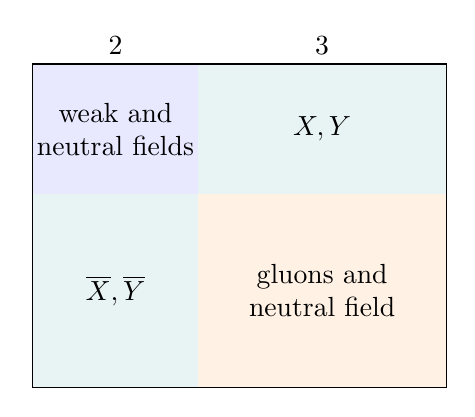
\begin{tikzpicture}[x=1.05cm,y=0.82cm]
  \draw[thick] (0,0) rectangle (5,5);
  \draw[thick] (2,0) -- (2,5);
  \draw[thick] (0,3) -- (5,3);
  \fill[blue!9] (0,3) rectangle (2,5);
  \fill[orange!10] (2,0) rectangle (5,3);
  \fill[teal!9] (2,3) rectangle (5,5);
  \fill[teal!9] (0,0) rectangle (2,3);
  \node[align=center] at (1,4) {weak and\\neutral fields};
  \node[align=center] at (3.5,1.5) {gluons and\\neutral field};
  \node[align=center] at (3.5,4) {\(X,Y\)};
  \node[align=center] at (1,1.5) {\(\overline X,\overline Y\)};
  \node[above] at (1,5) {\(2\)};
  \node[above] at (3.5,5) {\(3\)};
\end{tikzpicture}
\caption{Structure en blocs \(2\oplus3\) du champ de jauge de \(SU(5)\). Les blocs hors diagonale relient les leptons aux champs colorés.}
\label{fig:l10-gauge-blocks}
\end{figure}

Avec la convention \(Q=T_3+Y\), le doublet faible coloré dans ~\eqref{eq:l10-adjoint-sm} porte les charges \(-\tfrac13\) et \(-\tfrac43\) ; son conjugué porte les charges \(+\tfrac13\) et \(+\tfrac43\). Le cours appelle ces particules \(X\) et \(Y\), mais s’abstient explicitement de préciser quelle appellation correspond à quelle charge. La transition et la charge constituent le contenu invariant.

\begin{classroomqa}
\audiencequestion{Existe-t-il trois versions de chaque nouveau boson de jauge \(X\) ou \(Y\) ? \lecturetimestamp{00:41:28}}
\lecturerresponse{Oui. Une transition relie une composante de quark colorée à une composante leptonique sans couleur ; le boson échangé doit donc porter la couleur manquante. Les champs \(X/Y\) forment des triplets de couleur et peuvent émettre ou absorber des gluons.}
\end{classroomqa}

On n’observe pas de particules colorées comme états asymptotiques isolés. Les nouveaux bosons de jauge doivent se désintégrer ou hadroniser en combinaisons neutres en couleur, comme les quarks.

\section{Pourquoi le multiplet contient des quarks anti-down}

Les générateurs de \(SU(N)\) sont des matrices hermitiennes de trace nulle. Pour voir le lien avec le terme « spécial », écrivons un élément infinitésimal du groupe sous la forme
\begin{equation}
U(\epsilon)=e^{i\epsilon T}.
\end{equation}
L’unitarité donne \(T^\dagger=T\), tandis que
\begin{equation}
1=\det U=e^{i\epsilon\operatorname{tr}T}
\end{equation}
pour tout \(\epsilon\) donne
\begin{equation}
\operatorname{tr}T=0.
\label{eq:l10-traceless-generator}
\end{equation}

La charge électrique est une combinaison linéaire de générateurs. Sur la colonne de matière de ~\eqref{eq:l10-fivebar}, elle agit comme suit :
\begin{equation}
Q_{\overline5}
=
\operatorname{diag}
\left(0,-1,\frac13,\frac13,\frac13\right),
\qquad
\operatorname{tr}Q_{\overline5}=0.
\label{eq:l10-charge-fivebar}
\end{equation}
On a donc
\begin{equation}
0-1+3\left(\frac13\right)=0.
\end{equation}
Si l’on remplaçait les champs anti-down par des champs down, on obtiendrait plutôt
\begin{equation}
0-1+3\left(-\frac13\right)=-2,
\end{equation}
ce qui ne peut pas être la trace d’un générateur de \(SU(5)\). L’affectation apparemment étrange des anti-down est donc imposée par la structure du groupe.

\section{Les dix fermions restants}

Les dix autres champs proviennent d’un tenseur antisymétrique à deux indices. Dans la convention standard, il s’agit de la partie antisymétrique de
\begin{equation}
\mathbf5\otimes\mathbf5
=\mathbf{15}_S\oplus\mathbf{10}_A.
\label{eq:l10-five-five}
\end{equation}
Le cours le construit en écrivant temporairement les nombres quantiques conjugués :
\begin{equation}
\chi=
\begin{pmatrix}
\nu^c\\
e^c\\
d_r\\
d_g\\
d_b
\end{pmatrix}.
\label{eq:l10-aux-five}
\end{equation}
C’est un artifice de calcul pour former des produits de représentations, et non l’affirmation qu’il existe un second quintuplet physique de particules composites.

Posons
\begin{equation}
\Psi^{ij}=-\Psi^{ji},
\qquad
i,j=1,\ldots,5.
\label{eq:l10-antisym-ten}
\end{equation}
Tous les éléments diagonaux sont nuls, et le triangle inférieur est fixé par le triangle supérieur. Ainsi,
\begin{equation}
\dim\mathbf{10}
=\binom52
=\frac{5\cdot4}{2}
=10.
\label{eq:l10-ten-count}
\end{equation}

La charge électrique d’un élément est la somme des charges associées à sa ligne et à sa colonne dans ~\eqref{eq:l10-aux-five}. On obtient immédiatement \(e^c\) dans la case faible--faible, des quarks down et up dans les blocs faible--couleur, et des champs anti-up dans le bloc couleur--couleur.

\begin{classroomqa}
\audiencequestion{Lorsque les étiquettes du positron et du quark down sont combinées, l’élément qui en résulte devrait-il être un boson \(X\) ? \lecturetimestamp{00:53:08}}
\lecturerresponse{Non. À ce stade, nous construisons la représentation des fermions, et non la représentation adjointe des bosons de jauge. Les charges s’additionnent selon \(1-\tfrac13=\tfrac23\) ; l’élément possède donc les nombres quantiques d’un quark up.}
\end{classroomqa}

Un choix cohérent de signes de couleur est
\begin{equation}
\Psi^{ij}=
\begin{pmatrix}
0 & e^c & d_r & d_g & d_b\\
-e^c & 0 & u_r & u_g & u_b\\
-d_r & -u_r & 0 & u_b^c & -u_g^c\\
-d_g & -u_g & -u_b^c & 0 & u_r^c\\
-d_b & -u_b & u_g^c & -u_r^c & 0
\end{pmatrix}.
\label{eq:l10-ten-matrix}
\end{equation}
Un changement de phase des champs modifie certains signes affichés, mais ni la représentation ni le contenu en particules.

\begin{figure}[htbp]
\centering
\includegraphics[width=0.83\textwidth]{lecture_10_figure_05.png}
\lectureframe{00:59:17.500}
\caption{La matrice de matière antisymétrique \(2\oplus3\), dégagée et vérifiée en cours avec ses éléments et ses étiquettes de couleur.}
\label{fig:l10-ten-board}
\end{figure}

\begin{classroomqa}
\audiencequestion{Faut-il écrire la représentation de dimension dix sous forme de matrice, ou peut-on la représenter par une colonne ? \lecturetimestamp{00:56:24}}
\lecturerresponse{Les deux sont possibles. On peut énumérer les dix composantes indépendantes dans une colonne, mais la matrice antisymétrique \(5\times5\) montre comment \(SU(5)\) agit sur ses deux indices et est donc bien plus informative.}
\end{classroomqa}

\begin{classroomqa}
\audiencequestion{Dans le bloc couleur--couleur, l’élément marqué \(u\) devrait-il en fait être un champ anti-up ? \lecturetimestamp{00:57:51}}
\lecturerresponse{Oui. L’étiquette au tableau est corrigée en \(u^c\), un champ anti-up gauche. Deux charges de base de type down s’additionnent pour donner \(-\tfrac23\), soit la charge électrique d’un quark anti-up.}
\end{classroomqa}

\begin{classroomqa}
\audiencequestion{Les couleurs ont été omises dans plusieurs éléments de la matrice. Sont-elles tout de même conservées ? \lecturetimestamp{00:58:05}}
\lecturerresponse{Oui. Les trois indices de couleur sont rouge, vert et bleu. Les étiquettes ont été supprimées uniquement pour alléger la présentation.}
\end{classroomqa}

Une paire antisymétrique de représentations fondamentales de la couleur se transforme comme une anti-couleur :
\begin{equation}
\wedge^2\mathbf3\simeq\overline{\mathbf3},
\qquad
(rg,rb,gb)\sim(\overline b,-\overline g,\overline r).
\label{eq:l10-anticolor}
\end{equation}
C’est pourquoi les trois éléments indépendants du bloc couleur--couleur forment précisément le triplet de couleur anti-up.

Une génération est maintenant organisée sous la forme
\begin{equation}
\overline{\mathbf5}\oplus\mathbf{10}.
\label{eq:l10-family}
\end{equation}
Il est remarquable que \(u_L\) et \(u^c_L\) figurent dans un même multiplet irréductible, tandis que \(d_L\) et \(d^c_L\), ou \(e_L\) et \(e^c_L\), appartiennent à des multiplets différents.

\begin{classroomqa}
\audiencequestion{Si les transformations de jauge agissent uniquement à l’intérieur de chaque représentation, comment une masse peut-elle relier des champs appartenant au cinq-barre et au dix ? \lecturetimestamp{01:00:40}}
\lecturerresponse{Les bosons de jauge ne font pas passer une représentation irréductible de matière dans l’autre. Les champs de Higgs et les couplages de Yukawa peuvent relier des représentations différentes tout en formant une interaction globalement invariante sous \(SU(5)\) ; lorsque le champ de Higgs acquiert une valeur moyenne non nulle dans le vide, ces interactions engendrent des masses.}
\end{classroomqa}

\section{Les bosons de jauge agissent comme des décalages}

Une fois la représentation assemblée, l’action d’un boson de jauge se lit comme un décalage entre ses composantes. Un boson neutre peut laisser une étiquette inchangée, un boson faible fait passer d’un indice faible à l’autre, un gluon fait passer d’un indice de couleur à l’autre, et un boson \(X/Y\) fait passer d’un indice faible à un indice de couleur, ou inversement. Les bosons de jauge chargés ont des antiparticules : chaque décalage possède donc un processus inverse.

Pour le tenseur antisymétrique, une transformation infinitésimale agit sur chacun des indices :
\begin{equation}
\delta\Psi^{ij}
=
i\epsilon
\left(
T^i{}_k\Psi^{kj}
+
T^j{}_k\Psi^{ik}
\right).
\label{eq:l10-two-index-action}
\end{equation}
Dans la représentation matricielle, le premier terme produit un déplacement vertical et le second un déplacement horizontal. Les étiquettes des constituants utilisées pour construire le tenseur ne sont qu’un moyen mnémotechnique ; ~\eqref{eq:l10-two-index-action} exprime exactement l’énoncé en théorie des groupes.

Les décalages faibles transforment \(d\) en \(u\) : c’est le processus au niveau des quarks qui sous-tend la désintégration bêta du neutron. Les décalages de couleur changent le rouge, le vert et le bleu sans modifier la saveur. Les décalages hors diagonale produisent un effet nouveau :
\begin{equation}
\begin{aligned}
d^c&\longleftrightarrow e,
& d^c&\longleftrightarrow\nu,\\
d&\longleftrightarrow u^c,
& u&\longleftrightarrow e^c,
\end{aligned}
\label{eq:l10-leptoquark-shifts}
\end{equation}
le champ \(X/Y\) approprié portant la différence de charge et de couleur.

\begin{classroomqa}
\audiencequestion{Que représentent les décalages entre les quatrième et cinquième composantes, et qu’en est-il d’un décalage entre la première et la quatrième ? \lecturetimestamp{01:10:36}}
\lecturerresponse{Le décalage entre les quatrième et--cinquième composantes change une couleur en une autre : c’est une transition par gluon. Un décalage entre la première et la--quatrième composante franchit les blocs faible et couleur ; c’est une des nouvelles transitions \(X/Y\).}
\end{classroomqa}

\begin{classroomqa}
\audiencequestion{Peut-on remplir explicitement un élément de la moitié inférieure de la matrice antisymétrique ? \lecturetimestamp{01:11:23}}
\lecturerresponse{Oui. Chaque élément du triangle inférieur est l’opposé de l’élément transposé du triangle supérieur. En remplir un rend la règle visible ; les remplir tous n’ajoute aucun nouvel état.}
\end{classroomqa}

\section{La conséquence dangereuse : la désintégration du proton}

Un boson \(X/Y\) peut coupler un quark à un lepton à un sommet, et deux champs de type quark à un autre. À des impulsions très inférieures à sa masse, intégrer ce boson lourd donne une interaction de dimension six, de la forme schématique
\begin{equation}
\mathcal L_{\mathrm{eff}}
\sim
\frac{g_5^2}{M_X^2}\,(qq)(q\ell)
+\text{h.c.}
\label{eq:l10-effective-proton}
\end{equation}
Elle viole séparément les nombres baryonique et leptonique, tout en préservant les combinaisons imposées par l’interaction de jauge unifiée.

Au tableau, on suit un quark down et un quark up dans l’échange du boson lourd. Le quark down devient un positron, le quark up devient un quark anti-up, tandis qu’un second quark up reste spectateur :
\begin{equation}
uud
\longrightarrow
e^++u\overline u.
\label{eq:l10-quark-decay}
\end{equation}
L’état initial est un proton. La paire \(u\overline u\) peut hadroniser en un pion neutre, ce qui donne
\begin{equation}
p\longrightarrow e^++\pi^0.
\label{eq:l10-proton-pion}
\end{equation}

\begin{figure}[htbp]
\centering
\includegraphics[width=0.82\textwidth]{lecture_10_figure_06.png}
\lectureframe{01:16:02.500}
\caption{Construction achevée au tableau de l’échange du boson lourd à l’intérieur d’un proton ; le quark up spectateur et le canal avec positron sont visibles.}
\label{fig:l10-proton-board}
\end{figure}

Le cours mentionne aussi \(p\to e^++\gamma\), où la paire quark--antiquark s’annihile par interaction électromagnétique. Ce canal subit une suppression électromagnétique supplémentaire par rapport à l’hadronisation directe.

Cette possibilité n’est pas un ornement facultatif du modèle. Dès qu’un groupe simple contient des générateurs qui relient quarks et leptons, on s’attend en général à des processus qui violent le nombre baryonique. S’ils se produisaient aux échelles de temps ordinaires des interactions faibles ou électromagnétiques, les noyaux, l’hydrogène et la matière macroscopique ne survivraient pas.

\section{Pourquoi le proton vit-il aussi longtemps ?}

\begin{classroomqa}
\audiencequestion{Le couplage qui produit un boson \(X\) est-il le même couplage unifié que celui utilisé par le reste du groupe ? \lecturetimestamp{01:18:34}}
\lecturerresponse{À l’échelle d’unification, oui. Une théorie de jauge simple fondée sur \(SU(5)\) possède un unique couplage de jauge \(g_5\). Les couplages de basse énergie de l’interaction forte, de l’interaction faible et de l’hypercharge diffèrent parce qu’ils évoluent différemment après la brisure de la symétrie unifiée.}
\end{classroomqa}

On ne peut pas choisir un couplage extraordinairement petit sans renoncer à la structure unifiée. Le propagateur lourd fournit la suppression disponible :
\begin{equation}
\mathcal A
\sim
\frac{g_5^2}{M_X^2}.
\label{eq:l10-amplitude}
\end{equation}
Le carré de l’amplitude introduit le facteur \(g_5^4/M_X^4\). L’analyse dimensionnelle et l’élément de matrice du proton complètent l’estimation du taux de désintégration :
\begin{equation}
\Gamma_p
\sim
C_{\mathrm{had}}\,
\frac{\alpha_5^2\,m_p^5}{M_X^4},
\qquad
\alpha_5=\frac{g_5^2}{4\pi},
\label{eq:l10-rate}
\end{equation}
où \(C_{\mathrm{had}}\) regroupe les facteurs de groupe, les effets de renormalisation et l’élément de matrice hadronique non perturbatif.

\editorialnote{Le cours isole la dépendance essentielle en \(g^4/M_X^4\) et précise que les facteurs de masse du proton sont omis. L’équation~\eqref{eq:l10-rate} rétablit la dimension de masse requise sans prétendre fournir un calcul précis de la durée de vie.}

\begin{classroomqa}
\audiencequestion{Le petit facteur \(g^4\), peut-être de l’ordre de \(10^{-8}\) dans l’estimation approximative faite en cours, suffit-il déjà à rendre la durée de vie assez longue ? \lecturetimestamp{01:25:13}}
\lecturerresponse{Non. Il contribue à la suppression, mais l’écart entre une durée caractéristique microscopique des interactions fortes et la limite sur la durée de vie du proton couvre bien davantage d’ordres de grandeur. C’est la puissance quatrième de la masse élevée qui doit fournir la suppression décisive.}
\end{classroomqa}

Si toutes les masses étaient de l’ordre de la masse du proton, l’unité de temps naturelle serait approximativement le temps que met la lumière à traverser un proton :
\begin{equation}
t_p\sim\frac{1\ \mathrm{fm}}{c}\sim10^{-23}\ \mathrm{s}.
\label{eq:l10-proton-time}
\end{equation}
La seule existence de protons primordiaux montre déjà que leur durée de vie dépasse l’âge de l’Univers, mais les recherches en laboratoire vont beaucoup plus loin. Le cours compare l’estimation microscopique à la limite expérimentale citée à l’époque :
\begin{equation}
\tau_p\gtrsim10^{33}\ \mathrm{yr}.
\label{eq:l10-lifetime-bound}
\end{equation}

Il n’est pas nécessaire d’observer un proton unique pendant tout ce temps. Si sa durée de vie était de \(10^{15}\) années, un échantillon de \(10^{15}\) protons produirait environ un événement par an. Plus généralement, pour \(N_p\) protons observés pendant une durée \(T\), le nombre de désintégrations attendu est
\begin{equation}
\langle n\rangle\simeq\frac{N_pT}{\tau_p}.
\label{eq:l10-event-count}
\end{equation}
Un détecteur contenant environ \(10^{33}\) protons est une grande cuve, et non un objet astronomique : la masse des protons eux-mêmes est de l’ordre de \(10^6\) kilogrammes. L’observation d’un tel échantillon transforme une durée de vie individuelle gigantesque en un taux d’événements mesurable ou en une limite inférieure plus contraignante.

En combinant ~\eqref{eq:l10-rate} et la contrainte sur la durée de vie, on obtient pour la masse du boson de jauge leptoquark une valeur de l’ordre de
\begin{equation}
M_X\sim10^{15}\text{--}10^{16}\ \mathrm{GeV},
\label{eq:l10-mx}
\end{equation}
où \(10^{16}\,\mathrm{GeV}\) est l’échelle de sûreté mémorable retenue dans le cours. Elle se situe plusieurs ordres de grandeur au-dessous de l’échelle de Planck et n’est donc pas automatiquement incompatible avec la théorie quantique des champs.

\section{Brisure de \texorpdfstring{\(SU(5)\)}{SU(5)} et échelle d’unification}

Les champs \(X/Y\) partagent avec les champs de jauge du Modèle standard un multiplet adjoint de \(SU(5)\). Une symétrie de jauge exacte et non brisée ne permettrait pas que certains membres aient des masses proches de \(10^{16}\,\mathrm{GeV}\) tandis que le photon et les gluons restent sans masse. La symétrie doit donc être brisée spontanément.

\begin{classroomqa}
\audiencequestion{Si la symétrie \(SU(5)\) n’était pas brisée, tous ses bosons de jauge seraient-ils sans masse ? \lecturetimestamp{01:29:37}}
\lecturerresponse{Oui, dans la théorie de jauge considérée ici. L’invariance de jauge interdit une masse commune explicite. Le mécanisme de Higgs peut donner une masse aux bosons de jauge associés aux générateurs brisés, tout en laissant sans masse les champs de jauge du sous-groupe non brisé.}
\end{classroomqa}

Le mécanisme de Higgs électrofaible illustre déjà ce schéma : il distingue le photon des bosons \(W^\pm\) et \(Z\). La grande unification exige un paramètre d’ordre distinct à haute énergie, qui distingue le bloc faible \(2\) du bloc couleur \(3\) et rend extrêmement lourds les champs hors diagonale \(X/Y\).

Par rapport à \(10^{16}\,\mathrm{GeV}\), même une masse de boson faible de \(100\,\mathrm{GeV}\) est négligeable. Bien au-dessus du seuil des particules lourdes, on peut négliger toutes les masses des bosons de jauge, et la symétrie complète \(SU(5)\) devient une bonne approximation. C’est ce que signifie une échelle d’unification : le monde de basse énergie ne présente pas visiblement \(SU(5)\), mais les processus suffisamment énergétiques deviennent insensibles aux différences de masse dues à la brisure de symétrie.

\section{Évolution des couplages}

Les couplages de jauge dépendent logarithmiquement de l’échelle d’énergie. En définissant
\begin{equation}
\alpha_i(\mu)=\frac{g_i^2(\mu)}{4\pi},
\end{equation}
l’évolution à une boucle prend la forme
\begin{equation}
\alpha_i^{-1}(\mu)
=
\alpha_i^{-1}(\mu_0)
-\frac{b_i}{2\pi}
\ln\!\left(\frac{\mu}{\mu_0}\right).
\label{eq:l10-running}
\end{equation}
Les coefficients \(b_i\) dépendent du groupe de jauge et de chaque particule suffisamment légère pour intervenir dans les boucles quantiques pertinentes.

\editorialnote{Pour comparer l’hypercharge aux couplages non abéliens dans \(SU(5)\), il faut donner à \(g_1\) la normalisation conventionnelle de grande unification. C’est l’origine des facteurs numériques de théorie des groupes mentionnés dans le cours.}

Aux énergies accessibles en laboratoire, les inverses des trois constantes de couplage sont différents. Dans l’ordre qualitatif présenté dans le cours, \(1/\alpha_1\) est la plus grande, car l’hypercharge est l’interaction la plus faible ; \(1/\alpha_2\) vient ensuite, et \(1/\alpha_3\) est la plus petite, car l’interaction forte est la plus intense. Les courbes aux énergies inaccessibles ne sont pas mesurées directement. Elles sont calculées à partir des valeurs observées à basse énergie, du spectre des particules et des diagrammes de boucles qui déterminent les fonctions bêta. Avec le contenu en particules du Modèle standard, elles deviennent presque des droites lorsqu’on les représente en fonction de \(\log\mu\).

\begin{figure}[htbp]
\centering
\includegraphics[width=0.74\textwidth]{lecture_10_figure_07.png}
\lectureframe{01:36:32.500}
\caption{Représentation au tableau des constantes de couplage de jauge inverses qui se rapprochent vers \(10^{16}\,\mathrm{GeV}\). La région entourée indique qu’elles ne se rejoignent pas tout à fait.}
\label{fig:l10-running-board}
\end{figure}

En dessous de l’échelle d’unification, la symétrie est brisée, le spectre des particules légères ne remplit pas des multiplets \(SU(5)\) complets et dégénérés, et les trois coefficients des fonctions bêta diffèrent. Les constantes de couplage évoluent donc à des rythmes différents. À haute énergie, on se demande si elles atteignent une valeur commune :
\begin{equation}
\alpha_1(M_{\mathrm{GUT}})
\stackrel{?}{=}
\alpha_2(M_{\mathrm{GUT}})
\stackrel{?}{=}
\alpha_3(M_{\mathrm{GUT}}).
\label{eq:l10-unification-condition}
\end{equation}

Avec le seul spectre du Modèle standard non supersymétrique, les droites se rapprochent vers \(10^{15}\)--\(10^{16}\,\mathrm{GeV}\), mais sans se rejoindre : l’écart reste notable. Le cours décrit leur accord comme étant de l’ordre de quinze pour cent. La coïncidence remarquable est que cette échelle est aussi celle qu’exige la stabilité du proton.

\section{Une dernière question sur le neutron}

\begin{classroomqa}
\audiencequestion{Si le quark up spectateur dans le diagramme de désintégration du proton était remplacé par un quark down, cela décrirait-il la désintégration du neutron, et le boson \(X\) jouerait-il un rôle ? \lecturetimestamp{01:36:40}}
\lecturerresponse{Cela définirait un canal neutronique de grande unification, tel que \(n\to e^++\pi^-\), mais ce ne serait pas la désintégration habituelle d’un neutron libre. La désintégration bêta ordinaire du neutron est \(n\to p+e^-+\overline\nu_e\) et procède par l’interaction faible. Si l’ordre des masses du proton--neutron était inversé, la stabilité bêta le serait aussi, tandis que le canal de grande unification, beaucoup plus lent, pourrait subsister.}
\end{classroomqa}

Cette distinction sépare la cinématique de la nouvelle interaction. Lequel des deux nucléons se désintègre par bêta dépend de la différence de masse entre le proton--neutron ; la violation du nombre baryonique due à l’échange de \(X/Y\) est un mécanisme distinct, extrêmement supprimé.

\section{La supersymétrie et une perspective plus large}

L’ajout d’un spectre de partenaires supersymétriques modifie les coefficients des fonctions bêta dans l’équation~\eqref{eq:l10-running}. Dans le cours, les trois constantes de couplage extrapolées se rejoignent alors avec une précision d’environ un pour cent. Cela ne prouve ni la supersymétrie ni la grande unification, mais c’est la raison empirique pour laquelle ces deux idées sont souvent abordées ensemble.

Les multiplets de matière peuvent être unifiés davantage encore. Dans
\begin{equation}
SO(10)\supset SU(5),
\end{equation}
une représentation spinorielle se décompose ainsi :
\begin{equation}
\mathbf{16}
\longrightarrow
\mathbf{10}\oplus\overline{\mathbf5}\oplus\mathbf1.
\label{eq:l10-so10}
\end{equation}
Le singulet est naturellement identifié à un antineutrino de chiralité gauche, ou, de manière équivalente, à la conjuguée de charge d’un neutrino de chiralité droite. Ainsi, les seize champs d’une famille étendue s’inscrivent dans un seul multiplet irréductible de \(SO(10)\).

Les expériences sur la désintégration du proton continuent de mettre cette idée à l’épreuve : en l’absence d’événement observé, elles repoussent la limite inférieure de sa durée de vie. Les modèles supersymétriques de grande unification ne prédisent pas une durée de vie universelle du proton : des champs lourds supplémentaires et des opérateurs dépendant des superpartenaires peuvent modifier le canal dominant et le taux sur une vaste plage de valeurs.

\editorialnote{Dans la grande unification supersymétrique, l’échange de bosons de Higgs en triplets de couleur peut engendrer des opérateurs de violation baryonique de dimension cinq, en plus de l’opérateur de dimension six dû au boson de jauge évoqué ici. Leurs coefficients dépendent fortement du spectre des particules lourdes, de la structure de saveur et des masses des superpartenaires ; cela explique pourquoi le cours met en garde contre l’idée qu’une durée de vie unique découlerait de la seule supersymétrie.}

La leçon qui demeure est celle d’une tension, plutôt que d’un verdict. La théorie des groupes réunit quarks et leptons avec une remarquable économie, l’évolution des constantes de couplage suggère une échelle commune élevée, et la supersymétrie renforce cet indice numérique. Cette même construction prédit aussi la conversion dangereuse de quarks en leptons. Toute version viable doit donc préserver cette élégance tout en assurant la stabilité du proton pendant une durée presque inconcevablement longue. Pour reprendre l’esprit de la conclusion du cours : puissent tous nos protons rester stables.
